\begin{frame}[t]{LABEL}
  \begin{columns}
    \begin{column}{0.4\textwidth}
      \centering
      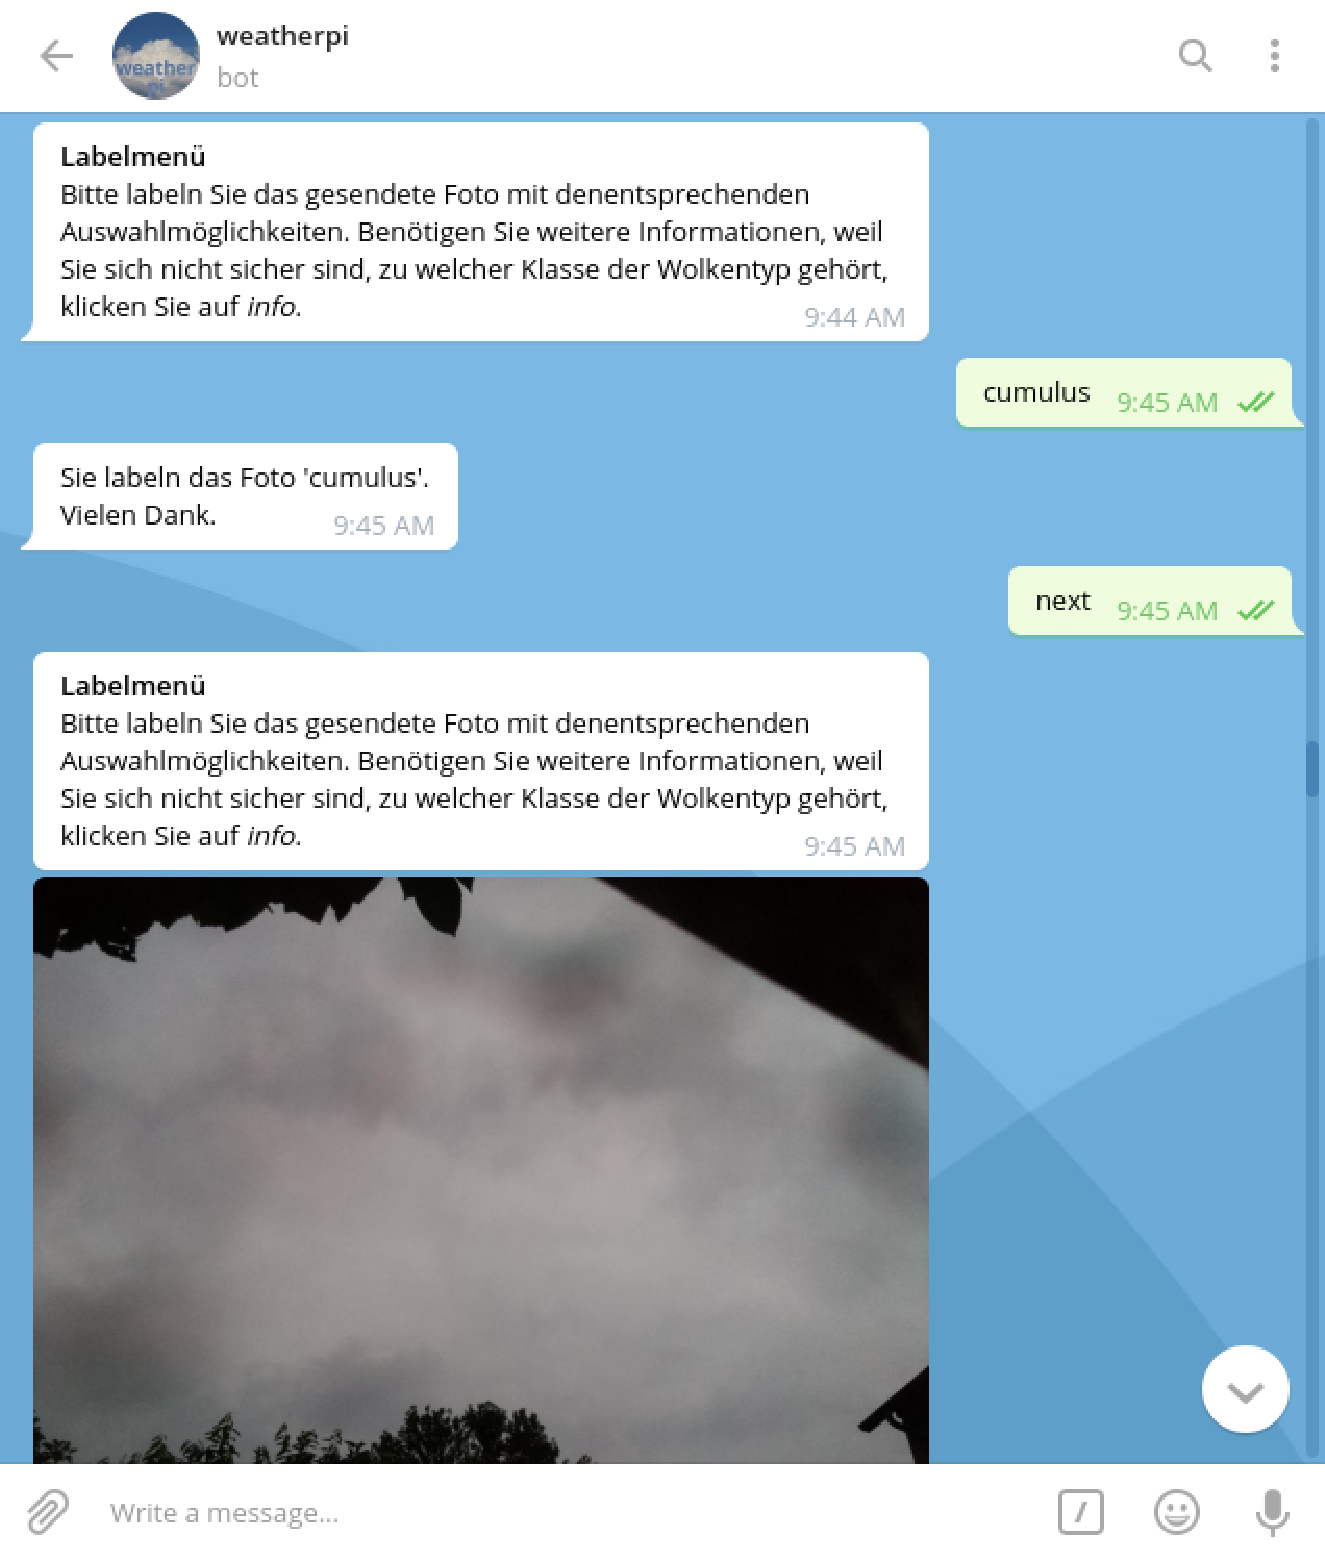
\includegraphics[width=\textwidth]{content/telegram_bot.pdf}
    \end{column}
    \begin{column}{0.6\textwidth}
      \begin{align*}
        &\hspace{15pt} \SI{4000}{Fotos} \cdot \SI{3}{Label} \cdot \SI{1}{\second} \\
        &\neq \SI{4000}{Fotos}
        \cdot \SI{3}{Label} \cdot \SI{15}{\second} \\
        &= \SI{25}{\hour\per Person}
      \end{align*}
      \begin{itemize}
        \item[$\rightarrow$] Ist das den Zeitaufwand wert?
          \begin{itemize}
            \item Daten + Label beliebig vereinbar
            \item GitHub
          \end{itemize}
        \item[$\rightarrow$] Parallele Threads überschreiben Label bei gleichzeitiger
          Nutzung
      \end{itemize}
    \end{column}
  \end{columns}
\end{frame}
